% http://www.r-bloggers.com/time-series-plots-in-r/
% http://www.fromthebottomoftheheap.net/2013/10/23/time-series-plots-with-lattice-and-ggplot/


% ------------------------------------------------------------
% ------------------------------------------------------------

%%%%%%%%%%%%%%%%%%%%%%%%%%%%%%%%%%%%%

% Section: Plots of TS in R 

\section[Time Series Plots]{Time Series Plots}
%%%%%%%%%%%%%%%%%%%%%%%%%%%%%%%%%%%%%

%\subsection{Univariate Plots}
%%%%%%%%%%%%%%%%%%%%%%%%%%%%%%%%%%%%%%

%\begin{frame}[fragile]
% \frametitle{Univariate Time Series Plot  \footnote{This section is from the SCC Mini-Course "Introductory Time Series \\ with R" by Irina Kukuyeva}}

%To plot one variables one at a time, use \ttfamily plot(): \normalfont 
%    \begin{columns}
%      \column{0.55\textwidth}
%		\begin{lstlisting}
%data(EuStockMarkets)
%dax<-EuStockMarkets[, 1]
%plot(dax)
%		\end{lstlisting}

%      \column{0.45\textwidth}
%       \begin{center}
%         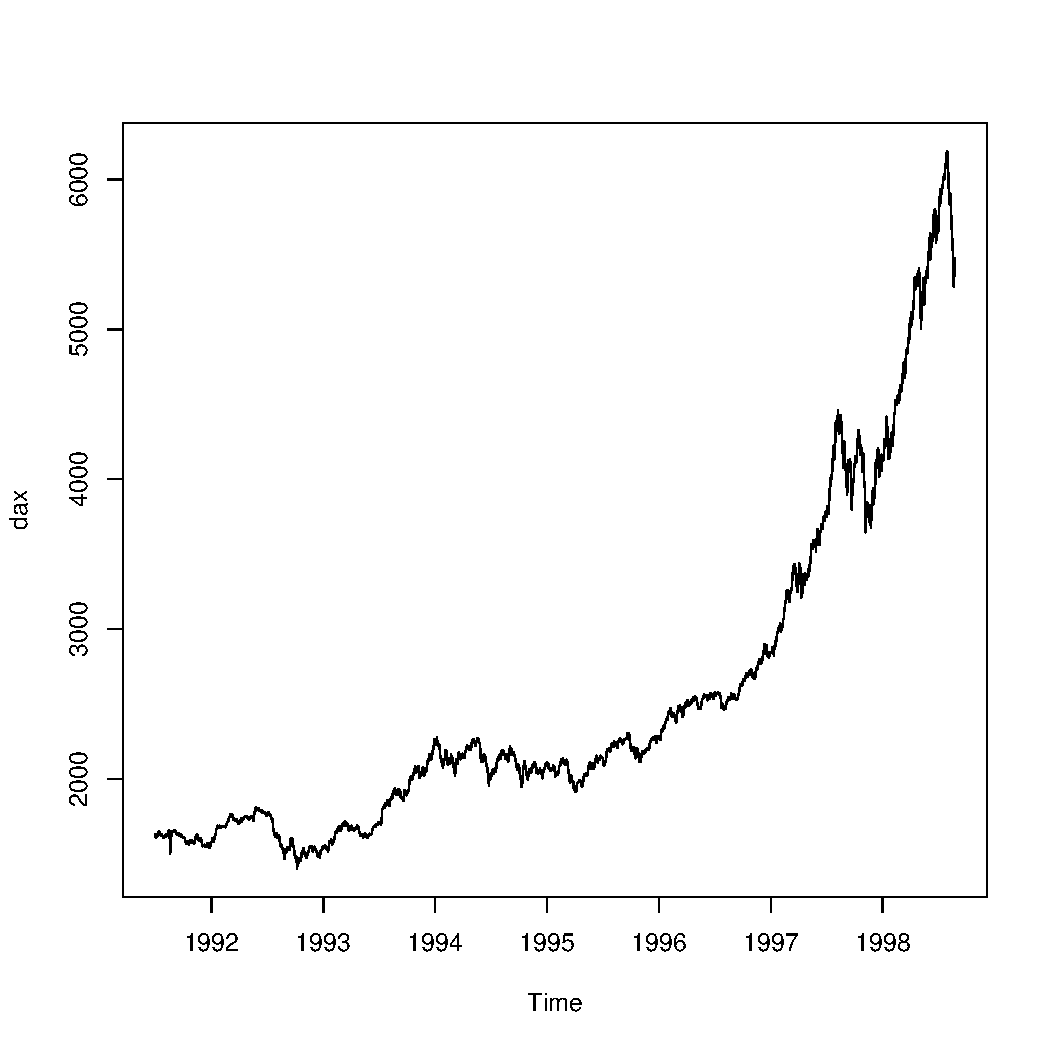
\includegraphics[width=0.95\textwidth]{images/daxPlot.pdf}
%        \end{center}
%      \end{columns}

%\end{frame}

%%%%%%% New frame
%\begin{frame}[allowframebreaks, fragile]
% \frametitle{Customizing the plot}

%To plot more than variables one at a time, use \ttfamily xyplot(): \normalfont
%		\begin{lstlisting}
%# After processing data as in Approach 1
%# load both libraries:
%library(lattice)
%library(zoo)
%data(EuStockMarkets)
%z<-EuStockMarkets
%xyplot(z, screen = c(1,1,1,1), col = 1:4, strip = FALSE)
%legend(1992, 5000, colnames(z), lty = 1, col = 1:4)
%		\end{lstlisting}

%       \begin{center}
%         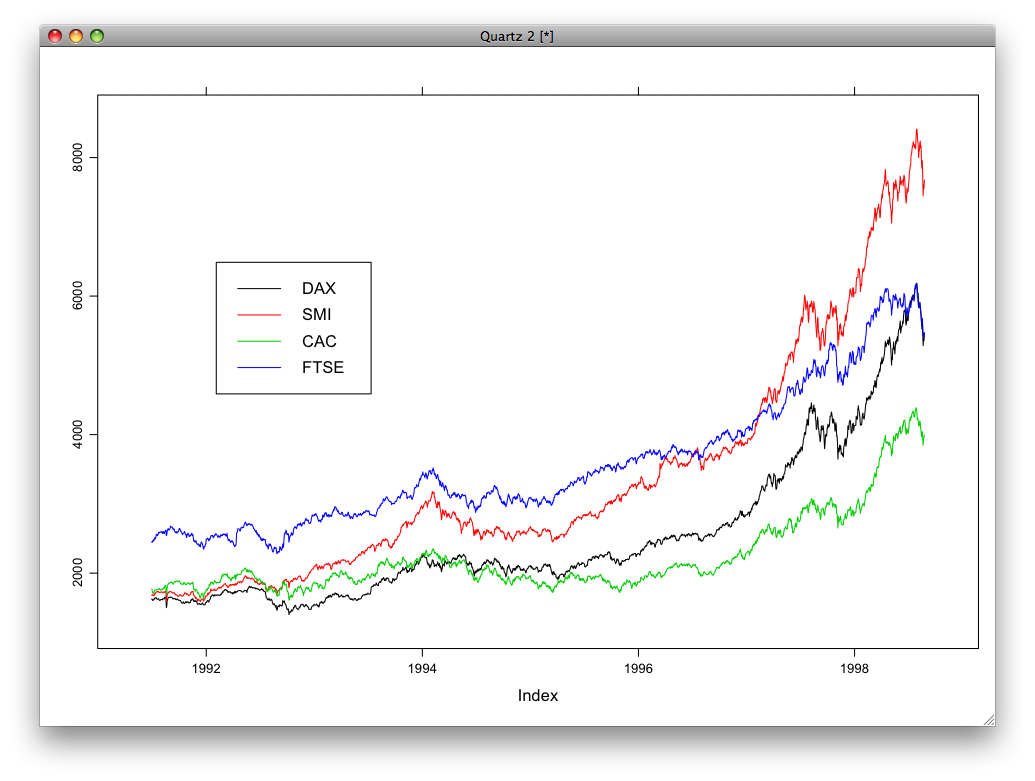
\includegraphics[width=0.85\textwidth]{images/stockPlot2}
%        \end{center}
%\end{frame}

%%%%%%%%%%%%%%%%%%%%%%%%%%%%%%%%%%%%%

\subsection{Multivariate Time Series Plots}

%%%%%%%%%%%%%%%%%%%%%%%%%%%%%%%%%%%%%

\begin{frame}[allowframebreaks, fragile]
 \frametitle{Multivariate Time Series Plots: Approach 1}

To plot more than variables one at a time, use \ttfamily xyplot()\normalfont [5]:
%\begin{itemize}
%	\item For documentation, go to: www.jstatsoft.org/v25/c01/paper 
%	\item Go to: http://www.biostat.jhsph.edu/$\sim$rpeng/RR/mvtsplot/
%	\item Copy the relevant R Code and paste it into the R Console. Press ENTER.
%	\item Plot your data
% \end{itemize}
		\begin{lstlisting}
### Step 0: Load any required packages
library(dplyr)
library(lattice)

### Step 1: Get data for one procedure
df_LA_CABG <- df %>%
  filter( 
    (County == "Los Angeles") & 
    (Procedure == "CABG") & 
    (Volume > 0) 
    )
    \end{lstlisting}

\newpage    
    \begin{lstlisting}
### Step 2: Visualize    
xyplot( Volume ~ Year | Hospital.Name, 
  data=df_LA_CABG,
  par.strip.text=list(cex=0.5),
  type="b",
  main="LA Coronary artery bypass grafting (CABG)"
  )
		\end{lstlisting}

\newpage
      %\vspace{-30pt} 
      \begin{center}
        %\hspace{-25pt}
         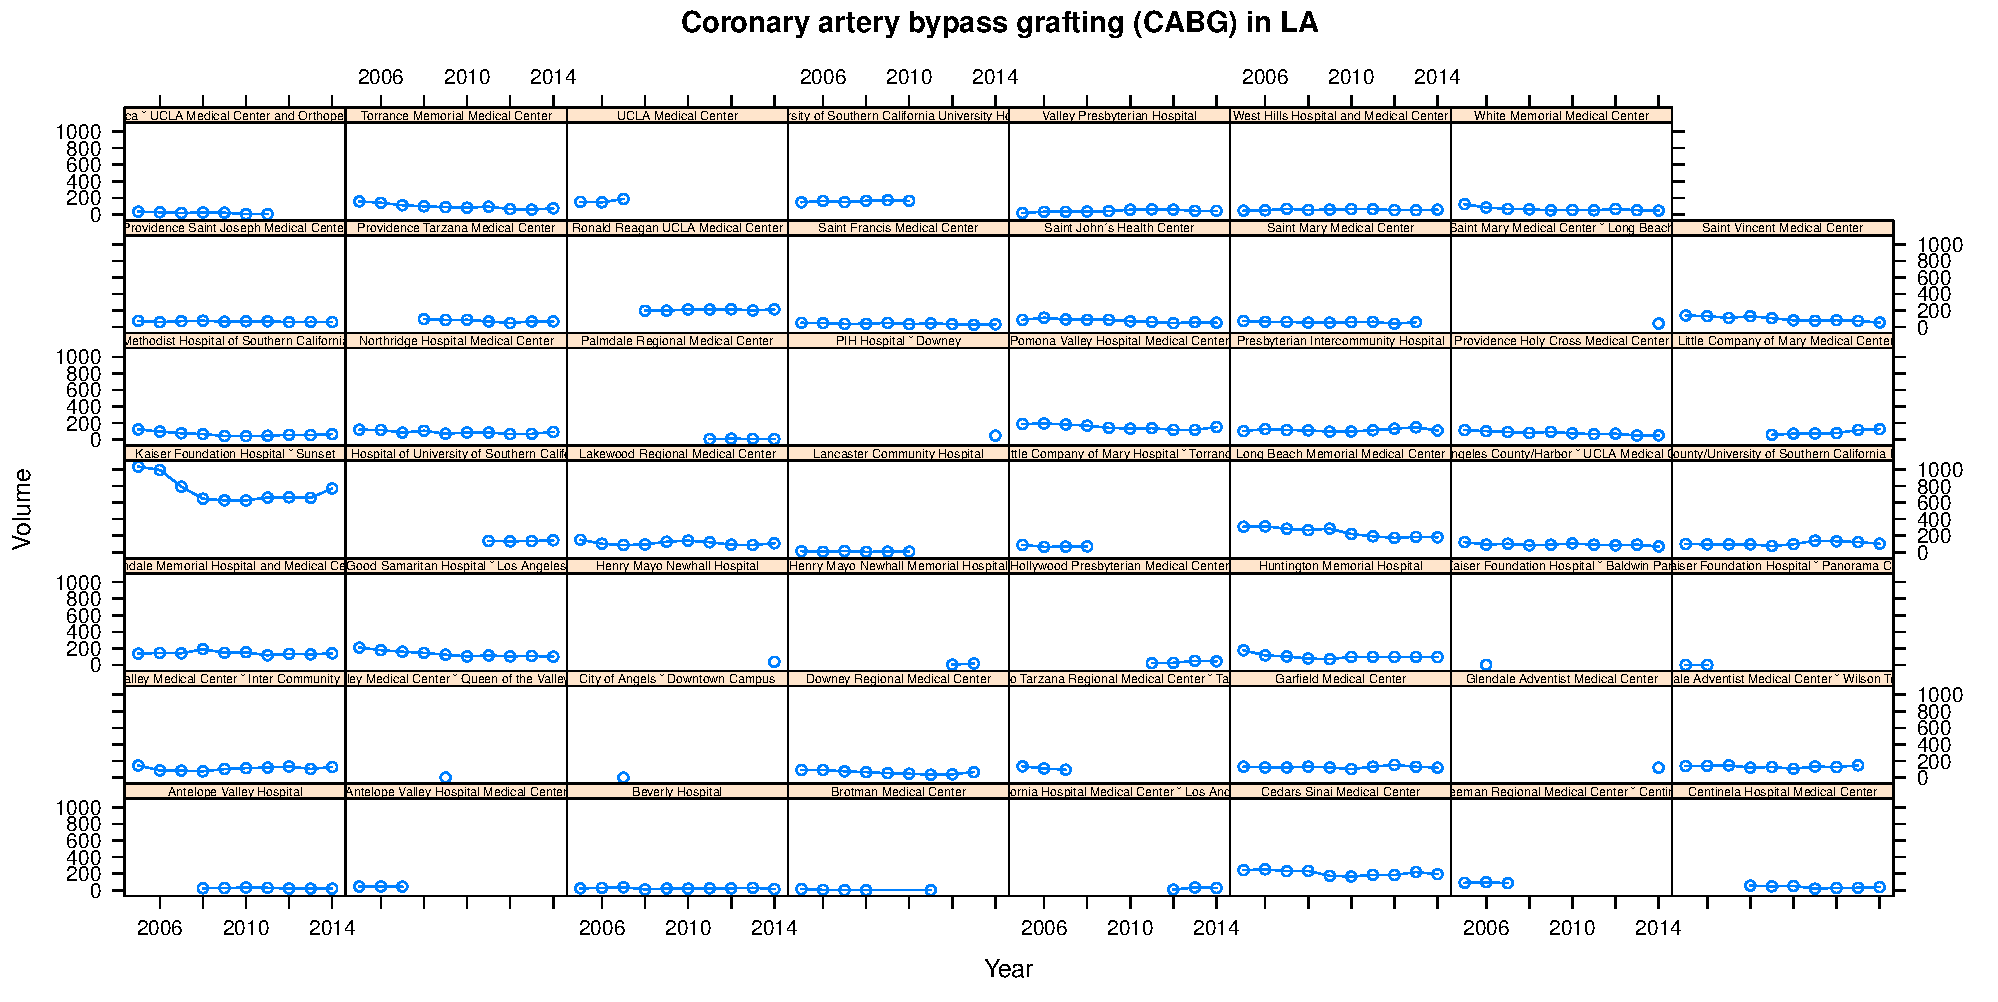
\includegraphics[width=1.05\textwidth]{images/timeseries_LA_CABG}
      \end{center}
\end{frame}

%---
\begin{frame}[fragile, allowframebreaks]
 \frametitle{Multivariate Time Series Plots: Approach 2}

Another way to plot more than one variable at a time, is via \ttfamily ggplot()\normalfont :

    \begin{lstlisting}
### Step 0: Load any required packages:
library(dplyr)
library(ggplot2)

### Step 1: Get data for one hospital:
df_Cedars <- df_clean %>%
  filter( Hospital.Name == 'Cedars Sinai Medical Center')
   \end{lstlisting}

\newpage
    \begin{lstlisting}
### Step 2: Visualize
ggplot( data = df_Cedars ) + 
  geom_line( aes(
    x = Year, 
    y = Volume, 
    linetype = Procedure) ) +
  scale_x_continuous( breaks=seq(
    from=2005, 
    to=2014, 
    by=3) ) +
  theme_classic() +
  ggtitle( "Volume of Procedures for Cedars Sinai Medical Center" )
   \end{lstlisting}

\newpage
       \begin{center}
         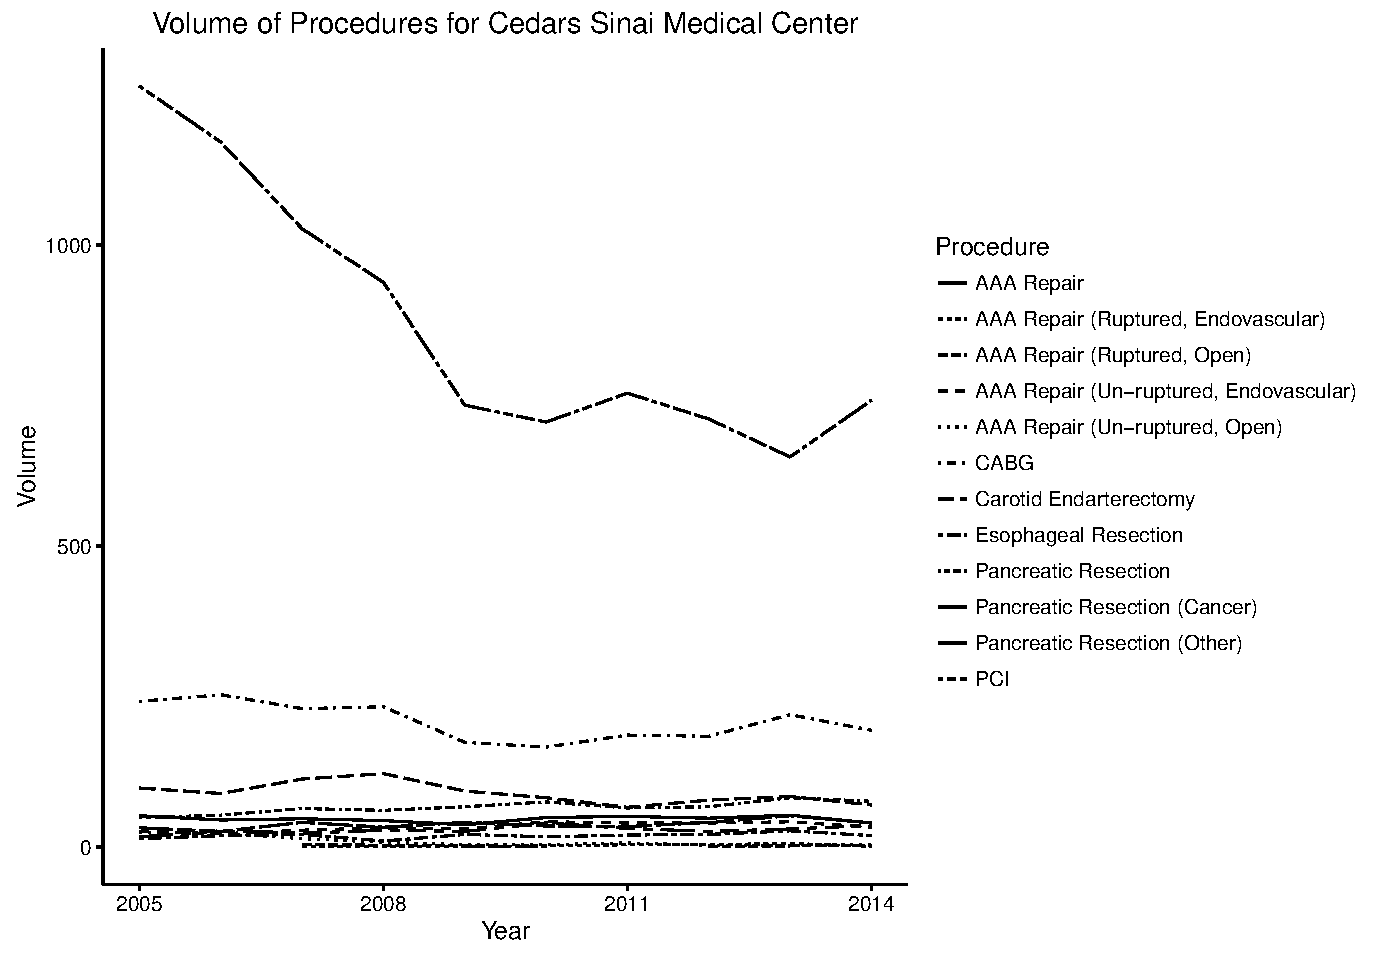
\includegraphics[width=0.9\textwidth]{images/timeseries_Cedars}
        \end{center}
\end{frame}

% % ------------------------------------------------------------
% % ------------------------------------------------------------
\subsection{Exercise II}
\begin{frame}[fragile]
	\frametitle{Exercise II}
	In the healthcare data set, what seems to be the most popular procedure in CA?\\
  \vspace{10pt}
  \noindent Hints: \small

    %%% TODO: show how to aggregate it by year and procedure

    \normalsize
\end{frame}
